\documentclass[12pt,letterpaper]{article}
    \usepackage[utf8]{inputenc}
    \usepackage[margin=0.5in]{geometry}
    \usepackage[english]{babel}
    \usepackage{amsmath}
    \usepackage{amssymb}
    \usepackage[tc]{titlepic}
    \usepackage{amsthm}
    \usepackage{graphicx}
    \usepackage[hidelinks]{hyperref}

    \urlstyle{same}

    \graphicspath{{./}}

    \title{On Leibniz's Attempt to Accommodate Freedom\\
    \vfill
    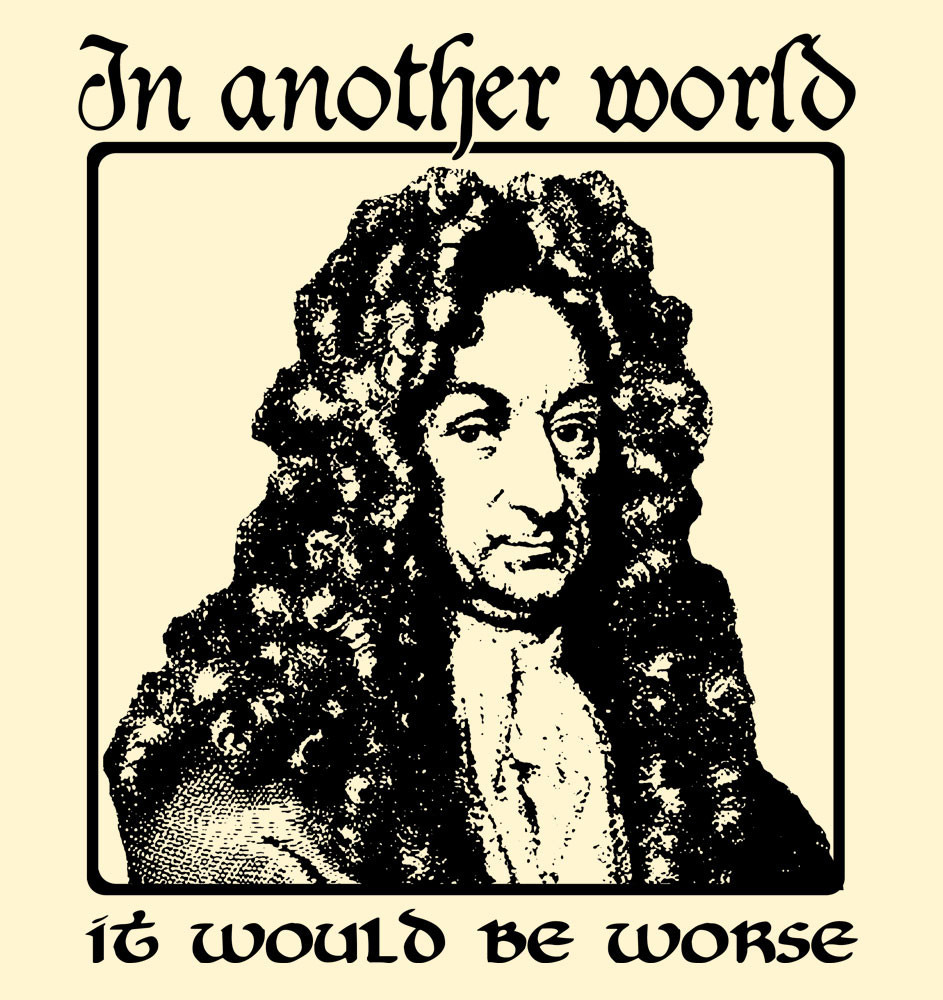
\includegraphics[width=400px]{leibniz.jpg}\footnote{I know we were not supposed to have a cover, but I found this image and I just had to use it.}
    \vfill
    }
    \date{November 2017}
    \author{Bernardo Meurer}

    \begin{document}
    \maketitle
    \newpage
    We begin by outlining Leibniz’s Concept-Containment Theory of Truth, in it he states that a statement is only true iff its concept-predicate is contained in its concept subject. Here, a statement is a sentence of form \(\mathcal S + \phi \), where \(\mathcal S\) is a subject, and \(\phi \) is a predicate, and his theory is stating \(\mathcal S + \phi\text{ is true} \iff \phi\in\mathcal C(\mathcal S) \), where \(\mathcal C(\mathcal S) \) is used to denote the \emph{concept-subject}, or \emph{the concept of \(\mathcal S \)}. Trivial examples of this are tautological statements, such as ``\(X\text{ is }X \)'', where the containment is axiomatic, and therefore evident.

    The theory becomes non-trivial in the case of contingent truths, such as ``Spinoza died in the Hague'', however Leibniz argues that any such truth can be reduced (through infinite analysis, although that is a later point) to primary truths, which again are self evident. One simple way to see that statement through Leibniz's theory is to take Spinoza's \emph{concept}, and think of it as a set composed of \(n \) elements \(\mathcal C(\mathcal S) = \{\alpha_1, \alpha_2, \ldots, \alpha_n \}, n\in\mathbb N \cup \{+\infty \} \), where one of said \(\alpha \)-elements is ``died in the Hague.'' If we now suppose for a moment that Spinoza did \emph{not} die in the Hague, we have a concept \(\mathcal C (\mathcal S')\) such that it contains every \(\alpha \in \mathcal C (\mathcal S)\) \emph{except} \(\alpha_k = \text{``died in the Hague.''}\) This, however, trivially implies \(\mathcal C(\mathcal S') \subset \mathcal C(\mathcal S) \) (where \(\subset \) denotes a strictly proper subset), which in turn gives us \(\mathcal C(\mathcal S) \neq \mathcal C(\mathcal S') \iff  \mathcal S \neq \mathcal S'\). In other words, had Spinoza \emph{not} died in the Hague, then that wouldn't be Spinoza at all that we are referring to, for simply being (in concept) Spinoza requires having died in the Hague\footnotemark[1].

    This theory brings forth an important issue, if all concepts are complete and static, that is to say no predicates can be added or removed from any concept, and they simply exist independent of their materialization (the concept of Spinoza existed before Spinoza existed) then do people have free will? If all we do is ultimately prescribed in our concept, which is independent of our existence, then how can there be any freedom? How are we not simply automatons following our instructions (described in out concept)?

    Leibniz's answer to this apparent flaw in his model is surprisingly simple. Firstly, as long as one acts spontaneously, which one does despite the predetermination from one's concept, then they act freely. Secondly, God could very well have created a world where Spinoza did not exist, and therefore he would not have died in the Hague, which implies that this truth is contingent. While the first argument is trivial, it is also unconvincing, I do not believe most people's definition of freedom is compatible with Leibniz’s, which makes the entire point of ``if you're not being forced you're acting freely'' to seem bogus, or at least to be committing some form of strawman fallacy. The second argument, however, requires deeper analysis to be made sense of and argued over.

    Firstly, we can see that for all concepts \(\mathcal C(S)\), there is a super-set \(\Omega = \mathcal P(\mathcal C(S))\), where \(\mathcal P\) denotes the power-set, which is composed of all possible versions of \(S\). In our previous statement, for example, we can claim that both \(\mathcal C(\mathcal S)\) and \(\mathcal C(\mathcal S')\) are contained in \(\Omega(\mathcal S)\), and in fact, we know that \(\mathcal S\) is such that both \(\mathcal C(\mathcal S)\) and \(\Omega(\mathcal S)\) are the largest possible, they aggregate the maximum number of elements and lesser forms respectively. This trivially implies that every other possible world is lesser to ours in completeness and complexity, for ours has all concepts as whole as they can be. Moreover, he also claims that we live in the ``best of all possible worlds,'' and his proof for it is as follows:
    \begin{equation*}
        \left.\begin{aligned}
               \text{God created this world} \\
               \text{He existed prior to its creation}\\
               \text{God is Free}\\
              \end{aligned}
        \right \}
        \text{God did not \emph{have} to create a world}
    \end{equation*}
    \begin{equation*}
        \left.\begin{aligned}
            \text{God acts with sufficient reason} \\
            \text{God complies with the principle of the best}\\
           \end{aligned}
     \right \}
     \text{Any world He creates is the best possible world}
    \end{equation*}
    So, although Leibniz claims that there is free will stemming from God's ability to create or not any such \(\mathcal C(S)\), he also ties that down. It seems that, despite his assertion of God's freedom, God \emph{must} create the most complete world, which is necessarily ours, and therefore he has no free will within his act of creation, but solely over creation itself, which again is incompatible with the general idea of freedom. In conclusion, Leibniz's argument, and his theory, does not truly accommodate free-will.

    \footnotetext[1]{A more through proof can be found at \url{http://meurer.xyz/articles/2017/10/25/on-leibnizs-truth}}
    %\footnotetext[2]{This proof can be shortly stated as \(\text{God created this world, He existed prior to his creation, and He is free} \implies \text{God did not have to create a world. God acts with sufficient reason, and complies with the principle of the best}\implies \text{Any world He creates is the best possible and since there is an infinite number of possible worlds, our is the best of them.} \)}
    \end{document}


